\usepackage{graphicx}

\documentclass{exam}
\usepackage[utf8]{inputenc}
\usepackage{amsmath}
\usepackage{graphicx}
\begin{document}


\title{Math TSI Evaluation Test}
\begin{center}
	\centering{\Large{     Del Mar College Math TSI Evaluation Test}}
	\newline
	\newline
	\fbox{\parbox{5.5in}{\centering
	Answer the questions below. You have as much time as is necessary. If you do not know the answer, leave the question blank.}}
\end{center}

\begin{flushleft}
	\makebox[\textwidth]{Student Name:\enspace\hrulefill}
	\newline
	\makebox[\textwidth]{Final Score:\enspace\rule{3cm}{0.5pt}}
\end{flushleft}
\vspace{5mm}

\begin{questions}
	\question Solve $x^2 = 4$.
	\vspace{2cm}
	
	\question Which of the following are equations of lines.
	\begin{checkboxes}
		\choice $y=mx + b$
		\choice $(y-y_{1}) = m(x-x_{1})$
		\choice $y = x^2$

	\end{checkboxes}
	
	\question Solve: $\frac{5}{3} + 1\frac{1}{2}$
	\vspace{2cm}

	\question Which of the following are polynomials?
	\begin{checkboxes}
		\choice $x^2$
		\choice $x^3 + y^5$
		\choice $\frac{y^3+7}{x}$
	\end{checkboxes}
	\vspace{2cm}

	\question Simplify $\frac{b^2+b}{b}$
	\vspace{2cm}

	\question What does PEMDAS stand for?
    \begin{checkboxes}
		\choice Please Excuse My Dear Aunt Sally
		\choice Pete Eats Mice During Autumn Showers
		\choice Pravioli Eravioli Mgive Dme Athe Sformuoli
		\choice Parenthesis Exponents Multiplication Division Addition Substraction
	\end{checkboxes}
    \vspace{2cm}

	\question What is the domain of the graph in the image to the left
	\begin{figure}
		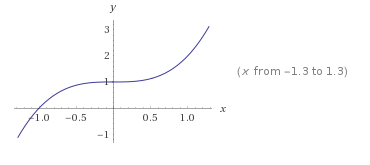
\includegraphics[width=2]{graph.png}
		\caption{Graph of $x^3 + 1$}
	\end{figure}

	\question How USB sticks can you buy if you have \$168, and a pack of 4 USBs costs \$12?
	\begin{checkboxes}
		\choice 56
		\choice 14
		\choice 168
		\choice 12
	\end{checkboxes}

    \question
	\begin{parts}
		\part Jasson has a NetFlix subscription which costs him \$13 a month. Create an equation which represents the
		amount that Jasson spends each month on his NetFlix subscription
			\begin{checkboxes}
				\choice $\frac{13}{x}$
				\choice $13^x$
				\choice $13x$
				\choice $13 + x$
			\end{checkboxes}
        \part Using this equation, calculate how much money Jasson spends in one year on his NetFlix subscription.
			\begin{checkboxes}
				\choice \$156
				\choice \$25
				\choice \$1.08
				\choice \$2 Million
			\end{checkboxes}
	\end{parts}
	\vspace{1cm}
	\question Factor Completely
	\begin{parts}
		\part $x^2 + 7x + 12$
		\vspace{2cm}
		\part $3x^2 + 5x + 2$
		\vspace{3cm}
		\part $5x^2 + 10x$
		\vspace{2cm}
		\part $4x^2 - 25$
	\end{parts}


	\question Expand and simply if possible $$(x + 3) (x + 5)$$
    \vspace{4cm}

	\question
	\begin{parts}
		\part $4^{\frac{1}{2}}$
		\vspace{1.5cm}
		\part $3x \cdot 3x \cdot 3y$
		\vspace{1.5cm}
		\part $(\sqrt[4]{128})^4$
		\vspace{1.5cm}
		\part $\sqrt[3]{27x^3}$
		\vspace{1.5cm}
    \end{parts}

\end{questions}
%\makebox[\textwidth]{Tutor Signature:\enspace\hrulefill}
\end{document}
